
\section{Evaluation of Project}
Evaluation of the project consisted of multiple stages ranging from verification of the functional requirements through simple black box testing to evaluation of refined mesh quality using methods provided by Dittmer \cite{DittmerMeshQualityMet}. 

\subsection{Validation Against Functional Requirements}
In order to validate the system against many of the functional requirements the system had to be run on a number of basic models with different input configurations. Having done this the results clearly demonstrate the system's ability to evaluate the quality of meshes using multiple refinement processes based on the stresses present within the structure and the specification of edges by a user. \\ 

\subsection{Validation of Software Quality}
\noindent
In the case of quality for the system's design and documentation evidence is provided in, (see appendices C, G and H)  to the requirements specified with the project submission containing detailed documentation in the form of a Deoxygen guide which shows the use of object oriented and functional software design as seen within the codebase. General applicability of functionality has also been demonstrated through evaluation using a variety of models and conditions when performing simulations.

\subsection{Unit Testing}
Holistic evaluation provided evidence of the overall system's effectiveness. Verification of individual components created trust in the accuracy of the results produced. Unit testing was also conducted from within Visual Studio (VS) using the NUnit framework and structured as a separate VS project. This guaranteed that the system was not able to interact with the tests and that testing was conducted through the class and function interfaces provided by the implemented solution. Tests were also grouped into classes with each test class corresponding approximately to one class within the system. Each test class then contains a number of test functions each of which performing the asserts necessary to deem its associated function as correct. This layout provided clear traceability from each item of functionality to its associated test making assessment of the test coverage much easier. Appendix B shows the visual studio test explorer containing the various tests. \\


\subsection{Software Quality and Management}
The software was developed using industry best practice including the use of appropriate variable naming, loose coupling of classes, use of abstractions and descriptive error messages which make the software easier to read and debug for any potential future developers. An effective version control strategy was also adopted by backing up all software to Github daily. \\

\noindent
Visual Studio also enabled calculation of various software quality metrics for the code base automatically. This made selecting parts of the codebase for refactoring much easier. Upon completion of the project the average maintainability index \cite{VisualStudioMaintainIndex} across all modules was 75 with the lowest score for any high level module being 60 and the highest 92. According to the Microsoft Developer Network (MSDN) website code with an index of between 0 and 9 indicates low maintainability, 10 to 19 indicates moderately maintainable and 20 to 100 high maintainability. \\ 

\subsection{Documentation}
The process of continuously writing descriptive documentation was important to the success of the project and was treated as an integral part of meeting the goals of the projects development methodology which aimed to reduce the systems complexity and improve readability. Through the writing Doc comments corresponding to every function within the codebase it was possible to generate documentation files automatically through use of the tool Doxygen. This allows anyone with the solution to view descriptions of each of its functions either in the codebase or alternatively through the manual produced automatically by Doxygen, for example see appendix. \\ 

 

\subsection{Evaluation Of Hybrids and Individual Methods of Refinement}
%To demonstrate the systems applicability to a variety of real engineering problems demanded the creation of several models resembling basic equivalents of real structures that are often analysed by FE methods.

%As a system designed to facilitate analysis of hybrid meshing techniques the ability to conduct detailed evaluation for a set of hybrids over multiple simulations demonstrates successful generality. \\

In order to validate the different methods of refinement it was important to carefully design tests for the system which would fairly measure its ability to compare a range of hybrid methods capable of performing meshing. \\ 

\noindent
Firstly it was important to test the various methods individually for at least one model in order to verify that each of the methods performs as expected, this is a key step in order to have trust in the results subsequently produced by the hybrids. When evaluating the hybrids the system also needed to be evaluated for several different FE models with varying simulation conditions. This demonstrates consistency in the results and the systems ability to work for a range of different model inputs. \\

\noindent
Hybrid performance evaluation should consider both good and potentially bad user input.  

\noindent
Three models were created in total for evaluation, with each of the models being a general simplification of a more complex model that could be expected within an industrial engineering setting. They model a suspension bridge, a part of a paper mill and a section of a generic cylinder. These models were developed specifically for the project although the paper mill and cylinder were based on two models used by Dolsak in order to train the ILP method when generating the rule set. Each model has a manually constructed low fidelity mesh built using LISA's graphical user interface. The models also have a set of forces applied to them which are required so that stress is induced within the simulation. Constraints are also assigned to surfaces as described under section 2.1. The results for the two models not analysed in this section (the cylinder and paper mill disk) can be found in appendices K and L. \\ 


\noindent
\textbf{Different Quality Edge Specifications: } Validation of edge specifications to reflect real world conditions was necessary, see 6.4 for heuristic edge specifications. Since the users specify the edges that determine the meshing focus they directly affect the final result of the process, it is therefore important to consider the results produced by the system for a variety of different potential users. The effects of good and bad edge specifications can be observed both in execution times for the simulations and in the system's ability to mesh accurately where required as seen in figure 15 and the mesh structure in appendix J. \\ 

\noindent
Since the three models were very different it was not possible to objectively compare the edge specifications for each of them. a basic criteria was therefore developed so that comparisons could be drawn. For each model four sets of edges were consequently constructed and given classifications of ``Best'', ``Good'', ``Ok'' and ``Poor'' With the following as general guidelines for defining each set: \\

\noindent
\textbf{Best: } Approximately five edges specified directly over or adjacent to those areas of known high stress within the model - input potentially generated by a user with a high degree of expertise in evaluating the specific type of structure. \\ 

\noindent
\textbf{Good: } Approximately three edges over or close to areas of high stress within the model - input potentially generated by a user with a high degree of general FE experience although potentially not specific to that type of structure. \\ 

\noindent
\textbf{Ok: } Three to five edges some near high stress and other not - representing a user with some experience but by no means an expert. \\ 

\noindent
\textbf{Poor: } Three to five edges none of which are close to areas of high stress - representing input as would be generated by an inexperienced user new to FE stress analysis. \\ 

\noindent
Not being a mechanical engineer it was necessary to find a way of defining what `Best' and `Good' looked like. To do this the traditional stress based refinement approach was run on each model to establish where high stress areas exist before using this to define a series of edge specifications of varying quality. Consequently it is only possible to objectively judge each of the different sets on the basis of the results they produce. These results would have had greater validity if time had allowed input from a range of practicing mechanical engineers. \\

\noindent
 
\subsubsection{Metrics Selections}
Due to the complex nature of finite element models there are a number of potential methods that can be used to evaluate the effectiveness of my approach. The metrics I eventually selected along with a description of what they indicate and why this was important to conclude the systems ability to meet its objectives is detailed below. \\ 

\noindent
\textbf{Average Maximum Internal Corner Angle: } This metric was cited by Dittmer \cite{DittmerMeshQualityMet}as one of the most consistent indicators by which to evaluate the quality of a mesh with gradual deviation from the optimum indicating a degradation in quality and the meshing processes inability to maintain quality and consequently ensure accuracy of subsequent results. Figure 3 show types of distortion, such as skewing, which can be detected by measuring the internal corner angle. \\ 

\noindent
\textbf{Execution Times: } Since it is important for all methods to run in a reasonable amount of time, measuring the increase in runtime with additional iterations provided a good indication of how costly each approach became and whether there were any points at which refined meshing became significantly more expensive. Comparing the execution times for the different approaches also indicates how much work each method is doing per iteration allowing the hybrids to be balanced, see section 5.8. \\


\noindent
\textbf{Average Stress Revealed for Each Iteration: } In order to measure the different methods ability to reveal stress over time the average stress across all the elements throughout the model is an effective metric to use. An increase in the average occurs as a result of more elements being placed on those areas of high stress and decrease occurring with creation of elements over areas of lower stress. Since this metric is a measurement of stress which is force over a given area stress is essentially a measure of pressure and as such the unit of measurement used is pascals. To simplify evaluation so as to take into account the different edge specifications the hybrid data below is based on the average values obtained for the heuristics when running all of the edge sets for the different models. \\ 


\subsubsection{Evaluation of Bridge Structure}
The suspension bridge model (see figure 19) consists of 196 elements of quad4 type and 212 nodes which can be considered coarse given the size of the structure. Four constraint points were specified at the base of each supporting column and strong forces were applied across the structure along the negative x axis. \\

\noindent
\textbf{Evaluating Individual Refinement Methods: } 
\noindent
 An important part of validating the proposed hybrid approach was to first evaluate each of the refinement methods individually and observe their performance. This then informs the weighting applied to each method to avoid either method dominating the results of the hybrid approach. To test the individual approaches effectiveness they were evaluated against the performance metrics defined in section 7.6.1 (i.e. time required to refine per iteration and average maximum internal element angle). The results of these validation tests are shown in figures 15 and 16. From these graphs it can be concluded that no individual method reduces the mesh quality and that both the individual methods spend approximately the same amount of time performing refinement per solve iteration meaning neither is overly favoured by a hybrid approach.
  

\noindent
 \\

% show angle and runtime



\begin{figure}[H]
  \centerline{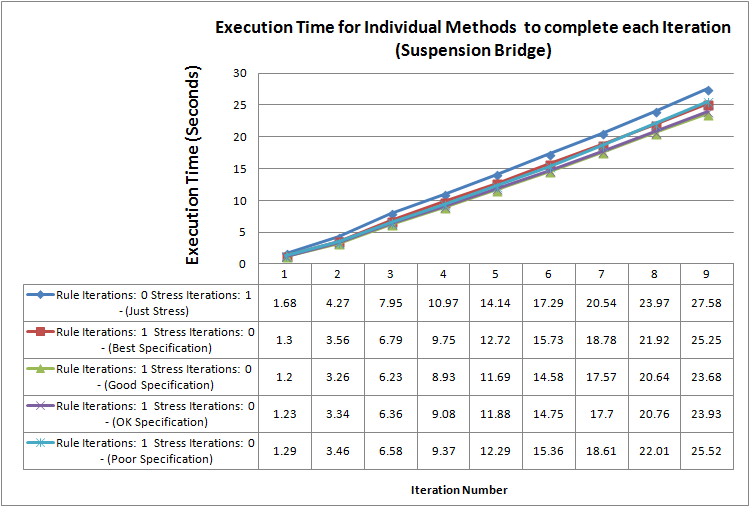
\includegraphics[width=110mm, scale=1]{../Graphics/FinalReportGraphs/ExecutionTimeIndividualMethodsSuspensionBridge.png}}
  \caption{Time taken to complete each iteration using the different methods}
  \label{fig:sub1}
\end{figure}  





 
\noindent
The maximum internal corner angles can be seen as improving linearly over time although with the greatest rate of improvement occurring during the first few iterations for each method before the average for the mesh approaches the optimum, which for elements of type Quad4 is 90 degrees. This means in general the refinement methods reduce skew present within the model through the creation of new elements and the calculated stress retains its accuracy. 

%This indicates that the refinement methods tend to reduce element skew within the mesh by effectively smoothing the mesh. This suggests that the results produced by the solver can be assumed to be at least if not more accurate after the mesh has been refined than before. This trend also extends to the other two evaluation models suggesting that the underlying subdivision process does not generate meshes that compromise the calculation of stress values for any input mesh.


\begin{figure}[H]
  \centerline{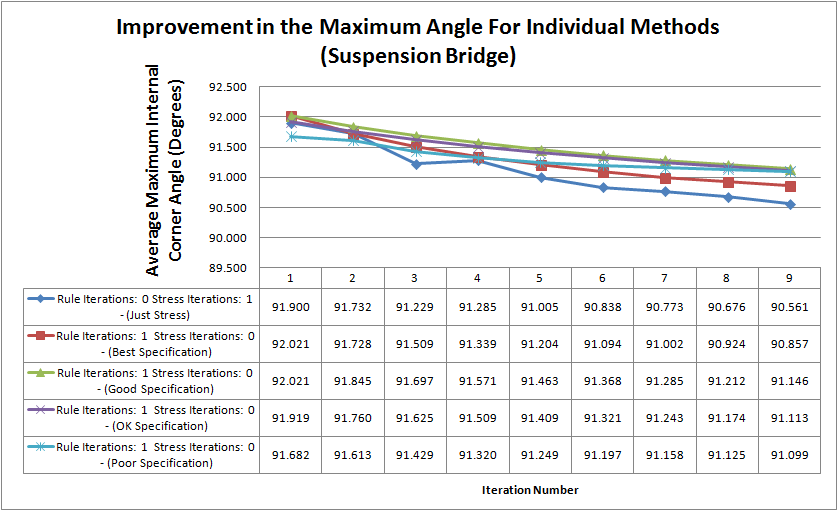
\includegraphics[width=110mm, scale=1]{../Graphics/FinalReportGraphs/AngleImprovementIndividualMethodsSuspensionBridge.png}}
  \caption{Approaching the ideal quad4 geometry for simulation data accuracy of 90 degrees using refinement with each of the different methods}
  \label{fig:sub1}
\end{figure}  

\noindent
%A key realisation having calculated the average maximum angles for the different methods was although Dittmers metrics helped to indicates that the results produced by the solver are accurate they do not actually demonstrate one refinement methods ability to mesh in more desirable areas than another while retaining a lower computational overhead through creation of fewer elements, an alternative metric was clearly needed in order to show this. A simple solution which proved highly effective was simply to calculate the average stress across all nodes. By calculating the average each method effectively achieved a high score for placing few elements directly over the high stress area while avoiding element creation over lower stress areas that would reduce the average.\\ 


\noindent
 

\noindent
\textbf{Evaluating Hybrid Refinement Methods: }
\noindent
When used on their own the heuristics (rules) based approach to FEM refinement revealed greater stresses than the traditional stress based approach. This is evidenced by figure 17 where after 6 iterations a heuristic approach had revealed stress levels up to the value of 6.3E+31 pascals whilst the traditional stress based approach revealed up to 4.5E+20 pascals. It can be concluded that there is demonstrative value in using a heuristic (rules) based approach regardless of whether used on its own or as part of a hybrid refinement strategy. \\ 

\noindent
Having completed analysis for each of the individual methods tests were run using hybrid strategies for each of the models. This produced results that indicate rapid overall improvement with regards to finding stress as can be seen below in figure 17 below. The improvement can be seen during the first few iterations in figure 18 before achieving a plateau.  The accuracy of the results were initially questioned with the values being extremely high, however Re-execution of the model with varying configurations including varying force and alternative constraints resulted in minimal differences. Conducting additional research revealed that this is not in fact an uncommon property of stress gradients within FE models \cite{StressConcerntration} as the calculated values for stress stress will trend towards infinity at points of serious weakness within a design when a high force is exerted and the stress is able to concentrate at particular points. A real structure would not be able to enduring stresses of these magnitudes and would break at these points of stress concentration before the stress calculated by the solver could actually occur.  Figure 19 below shows the bridge model undergoing relatively high stress at various points across the model but with rapid increase at specific points where structures join one another (highly focused red patches in 19b). \\


\textbf{\begin{figure}[H]
  \centerline{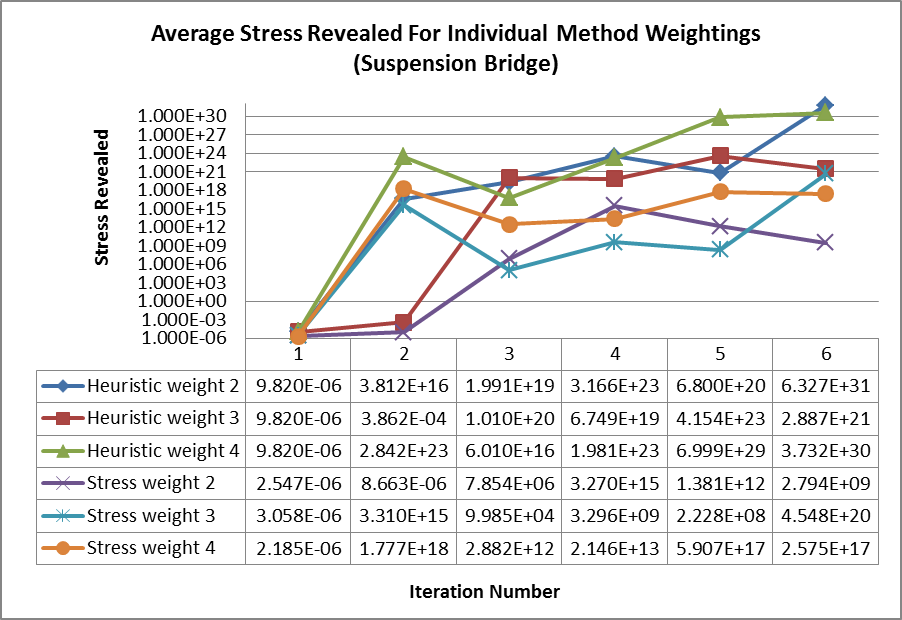
\includegraphics[width=110mm, scale=1]{../Graphics/Graphs/AverageStressesBridge/AverageStressRevealedForIndividualMethodWeightings.png}}
  \caption{Average stress revealed with different weightings for the individual methods}
  \label{fig:sub1}
\end{figure}}


\textbf{\begin{figure}[H]
  \centerline{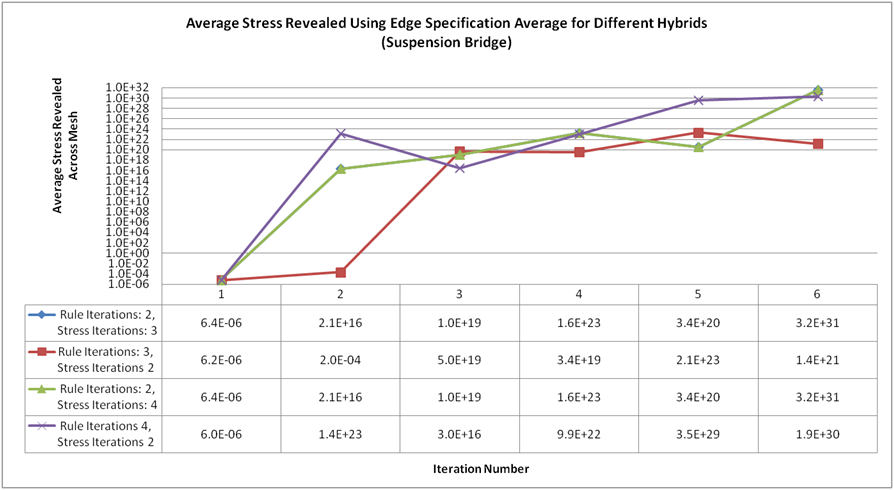
\includegraphics[width=110mm, scale=1]{../Graphics/FinalReportGraphs/AverageStressRevealedSuspensionBridge.png}}
  \caption{Average stress revealed using multiple iterations of the different hybrid methods over time}
  \label{fig:sub1}
\end{figure}}


\noindent


\noindent
Figure 19 indicates some unpredictability in the hybrid results i.e. when combining the individual methods. For example hybrid (3, 2) shows poor performance until iteration three while the other hybrid approaches, show similar accuracy to the individual methods. All the hybrid methods show greater consistency of results after iteration 3. \\ 

\noindent
When combining the heuristic and stress based approaches together to form a hybrid approach the level of stress found and the speed at which it was found was no worse than using the heuristics approach on its own. This is evidenced by comparing data from figure 19 (hybrid plots) against figure 17 (individual plots) i.e. after 6 iterations the hybrid approach had found stresses of value 3.163E+31 pascals against a figure of 6.32E+31 pascals for individual plots. \\ 

\noindent
From this observation it can be concluded that the influence of the heuristics on the overall hybrid approach is much greater than anticipated. Even when this affect is compensated for by using a hybrid strategy which heavily weights in favour of the stress approach (e.g. where heuristic rules weighting = 2, stress weighting = 4) the average stress after 6 iterations remains similar to a rules only approach. This suggests the need for further work to identify why this is occurring and then feed this back into the weightings for future development. \\

\noindent
Having run the model with the hybrids the coloured stress gradients across each structure can be inspected by an engineer, see figure 19 and appendices J below. LISA assigns colours to different ranges of stress based on the range of values within the model. In the majority of cases red areas represent those areas of highest stress followed by orange, yellow, green, light blue and eventually dark blue.  \\ 


%say something about how actually you want a bit of distribution
%\noindent
%Comparing the amount of improvement performed by both the stress and heuristic refinement processes with varying weightings that in general heuristics performed better than stress refinement although interestingly more weighting did not necessarily correlate to better results as can be be seen with heuristic weighting of two doing a better job than weighting four in the final iteration. \\

%../Graphics/BridgeCrossLoadingStress/bridgeStressBasic.png
\begin{figure}[H]
\centering
\begin{subfigure}{.5\textwidth}
  \centering
  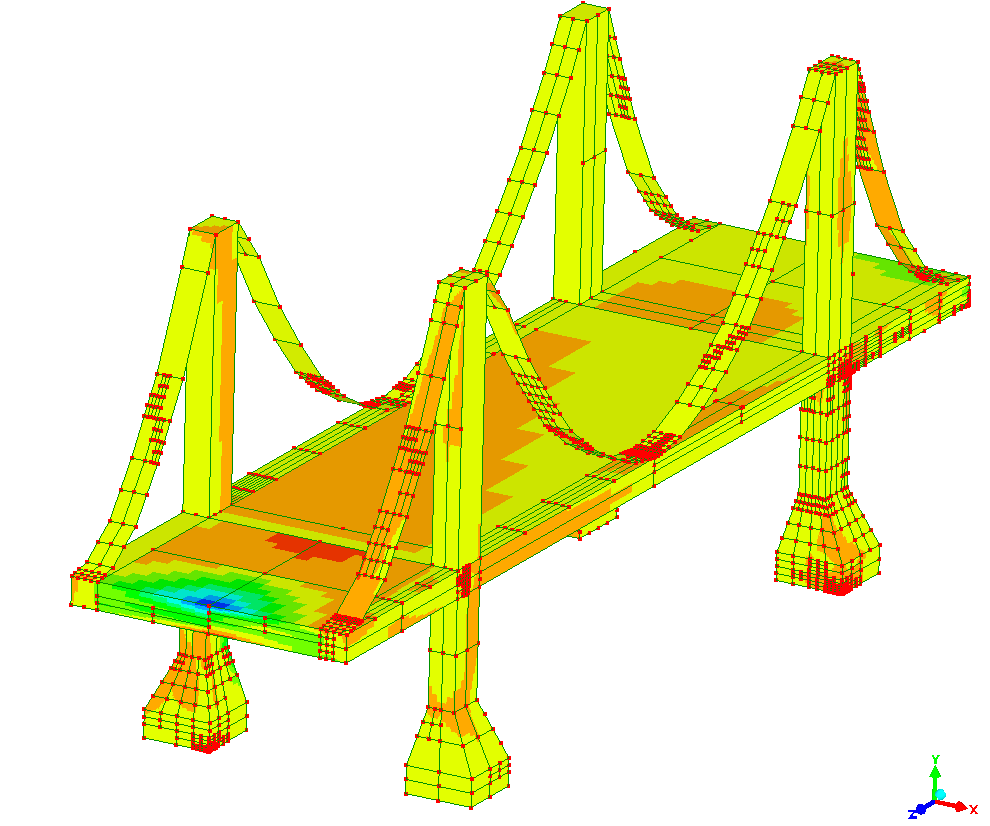
\includegraphics[width=0.9\linewidth]{../Graphics/BridgeCrossLoadingStress/Hybrid-best-3-2.png}
  \caption{Stress Revealed through the initial highly coarse bridge mesh without running any iterations for either method}
  \label{fig:sub1}
\end{subfigure}%
\begin{subfigure}{.5\textwidth}
  \centering
  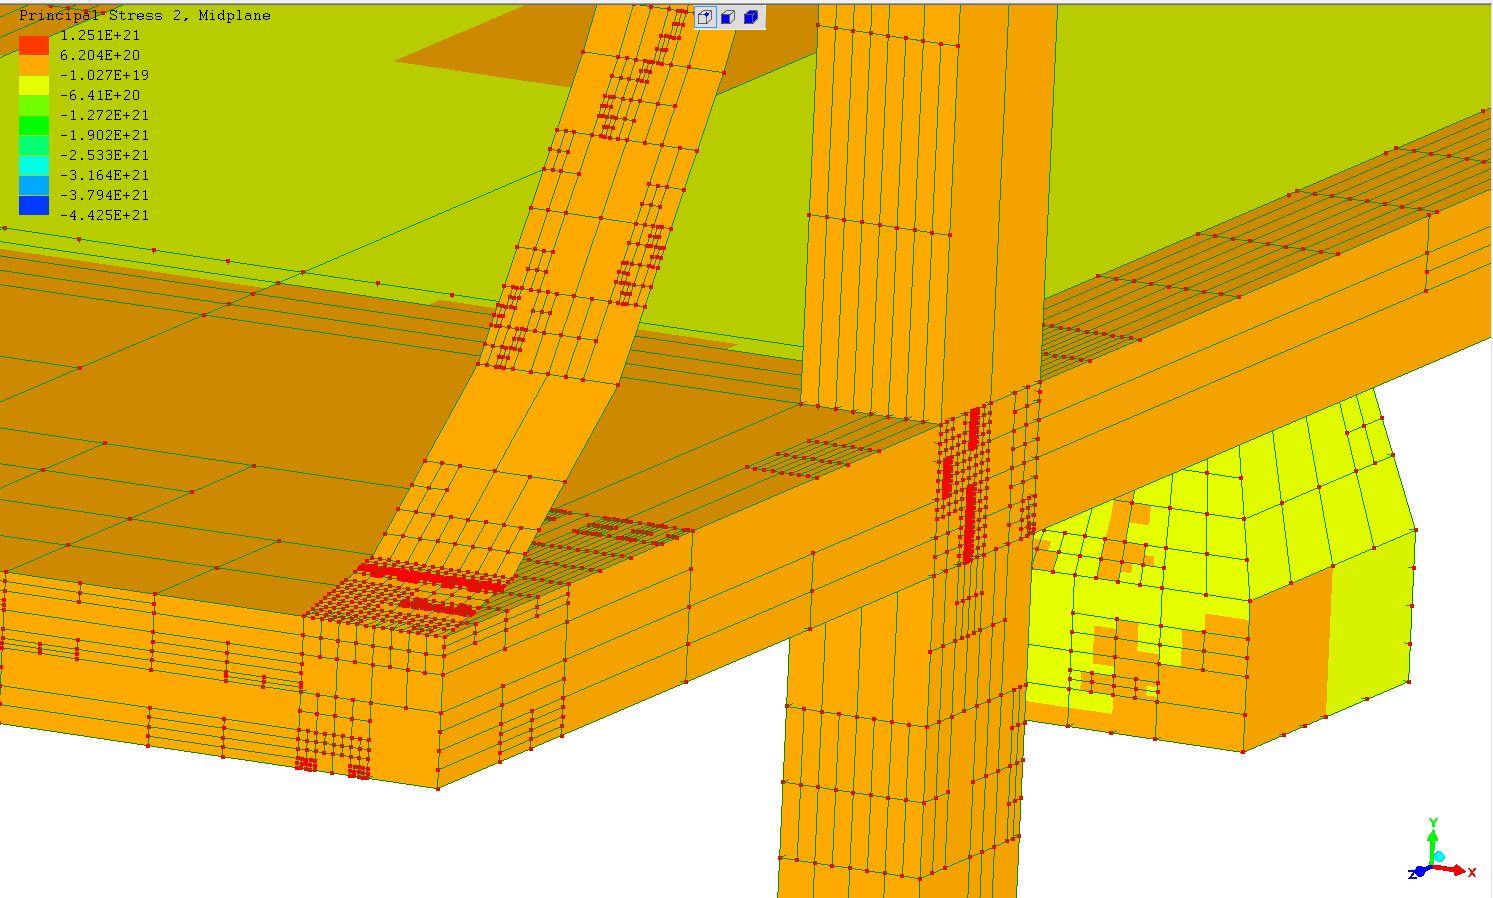
\includegraphics[width=0.9\linewidth]{../Graphics/BridgeCrossLoadingStress/BridgeCrossLoadingStress6-3-2.png}
  \caption{Meshing highly concentrated in those areas of the structure where the stress converges}
  \label{fig:sub2}
\end{subfigure}
\label{fig:test}
  \caption{Stress revealed within model after just 4 iterations with a heuristic stress method weighting of 3-2, edge heuristics also considered good in this case}
 \end{figure}



\noindent
In addition to the data summarised in this section of the report additional data collected for the various hybrid approaches applied to two other models is summarised in Appendices K and L. These results show how the hybrid approaches perform against the performance metrics identified in section 7.6.1 and provide reassurance that whilst the hybrid method cannot conclusively be demonstrated to calculate stress quicker than traditional methods the quality of the output (as measured by the performance metric) is as good as any other method used. 


\subsection{Strengths and Weaknesses}
The resulting system successfully satisfied both the functional and non functional requirements in addition to providing insights into the possibilities of a hybrid technique for effective finite element meshing, something that was optimistic at the start of the project but highly desirable. The project was well managed with all of the objectives being delivered as per the initial time plan, see appendix M. Quality was also maintained throughout the project by the application of good software engineering practice. \\

\noindent
The adoption of a modular architecture was a great great strength of the system allowing for a huge amount amount of potential extendability in the future and simplifying the ease with which both the individual methods could be combined to form new hybrid approaches. Although little focus has so far been given to the system's usability it could be developed and distributed as a public tool for experimentation with hybrid meshing with limited additional effort. Another highly flexible aspect is the system's ability to accept any heuristic definition in terms of edges within a mesh structure. Theoretically this means the final system is also capable of using the same types of edge specifications for any type of FE analysis such as fluid flow or heat transfer given a corresponding rule set to inform the refinement of the mesh. \\


\noindent
A downside of the current design is the need for the user to manually specify the edges by manually entering data into the JSON input file which is both time consuming and prone to error despite the relatively small size of the models analysed in this dissertation. Comparing the size of these with those used in industry it is clear that this process is simply not practical for engineers conducting large scale FE analysis. To address this better tools are required that will allow engineers to automatically generate edge specifications quickly, most likely through some GUI or a bespoke high level language capable of combining knowledge about the mesh structure and different types of edges to generate specific rules. Again this is beyond the scope of the project and would likely be a dissertation in its own right. \\


\noindent
Although the system had a strong subsystem and class level architecture many of its weaknesses could be attributed to needing to prioritise the ability to perform rapid prototyping over efficient implementation of the various algorithms and methods described in this dissertation. Much of this a consequence of overusing the functional programming capabilities within the C\# LINQ library. Widespread adoption of functional programming practices was stated as a desirable aspect of the final system implementation within the non-functional requirements in order to simplify the design and reduce unnecessary state, see appendix A. This was largely adhered to with significant use of lambda and higher order functions throughout the codebase. However, in the later stages of the project it became apparent that in many cases reliance on these features over more traditional programming constructs such as loops and conditions resulted in reduced readability of the code and a potential reduction in speed for implementations of the algorithms described in this dissertation.


%%%%%%%%%%%%%%%%%%%%%%%%%%%%%%%%%%%%%%%%%%%%%%%%%%%%%%%%%%%%%%%%%%%%%%%%%%%%%%%%%%%%%%%%%%%%%%%%%%%%%%%%%%%%%%%%%%%%%%%%%%%%%%%%%%%%
\section{Further Work}
This section details some areas which given additional time would be investigated, if not implemented. Each of these areas would hopefully provide some benefit in assisting to further demonstrate the possibilities of hybrid methods.

\subsection{Gathering Feedback From Experienced Engineers}
Approaching the end of the project it became clear that in order to better identify the systems strengths and weaknesses would require additional user testing by engineers who have experience conducting this type of analysis. Feedback from engineers with applied industrial experience along with that of academics would have allowed for a more conclusive analysis of the system and its ability to work across a greater number of general case scenarios. No user feedback was obtained within the duration of the project as a result of time constraints and the complexity inherent in simply implementing and validating the project for a selection of basic models. As such even if time had been available the ethical clearance required to collect user feedback at the start would need to have been acquired.


\subsection{Improving Usability Through A Web Interface}

\noindent
Lack of straightforward portability for the system was one factor that would have made it difficult to get feedback from industry, an alternative approach would be to develop a web interface so as to allow users to easily interact with the system externally. This approach would allow engineers to submit feedback digitally which could then be aggregated from a much greater range of users separated geographically. \\\ 

%Instead by facilitating interaction with the system by means of a web interface the engineers would be able spend as little or as much time as they like experimenting with 

\noindent
To use the web interface an engineer would simply need to submit a model they have already created  along with a JSON file containing edges they have designated as important for their model. LISA supports imports from multiple CAD formats including the Standard for the Exchange of Product model data (STEP) and Initial Graphics Exchange Specification (IGES)) \cite{LISAManual}. Upon receiving the request the web server would run the system using their input data and having finished allow them to download the re meshed models along with the calculated stress data for analysis.


\subsection{Added Sophistication of Hybrid Generation}
It has been shown the system can be used to effectively execute and evaluate fixed combinations of different methods each weighted in a predefined manner. This is a simple approach to demonstrating the working concept, however in reality the optimum meshing strategy is likely to be some fuzzy function of several meshing approaches with gradient weighting. As such this would be an exciting direction in which to take the project in future and would greatly increase the experimentation flexibility of the overall system.


\section{Project Conclusion and Personal Reflections}
%While conducting research, development and implementation for the project I have worked methodically to best understand each problem as and when they occur and consider each of the possible solutions before committing to one. I feel this approached has saved me much time and has forced me to reach a better view about what exactly each subsystem should do and how to implement it. In hindsight if I were to repeat the first part of the project again I would have organised my time differently to spend less of it focussed on the details of coursework assignments for other modules into making further progress on the implementation of the rule system.

%\noindent
%Overall I felt the project was a success. The final software solution was evidently capable of facilitating execution of the specified functions and therefore allowed comparison to be made of both heuristic and stress based mesh refinement techniques. Not only did the final system allow this comparison for the two specific approaches selected, it provided a flexible framework allowing experimentation for hybrid meshing using any two meshing approaches. \\ 

\noindent
Having used the system to successfully evaluate a range models and compare two individual methods for finite element meshing along with hybrid composites of the two it has been shown that the project has been delivered to meet each of the three main objectives outlined under ``Description Of The Work'', see section 4. The delivered system has been demonstrated capable of effectively evaluating meshing approaches using both a traditional refinement approach and one derived from the domain of AI with effective comparisons between each. Simulation results from the suspension bridge above and the paper mill disk and cylinder (appendices K and L) have shown that there are significant potential benefits of using an alternative method such as an expert system in conjunction with traditional stress based refinement and that this can be applied without degradation of quality to the original mesh geometry. Although unlikely that an alternative refinement process will supersede stress based refinement in the near future the high computational cost for large models and the demonstrated potential of alternatives supports the case for conducting further research and development in this area. \\


\noindent
From my own perspective I wanted to use this project as an opportunity to improve my understanding of a technology that I previously had limited knowledge of through its use on my industrial placement year. My prior experience with FE analysis was very much confined to that of a typical engineer making use of the method through a licensed desktop application with many of the technicalities that are of most interest to a computer scientist hidden. I therefore found the project highly useful as an opportunity to learn more about the underlying processes through both research and practical experimentation. As a means of facilitating my personal learning  I therefore also consider the project a success. \\ 

\noindent
Despite working on larger software projects during my year within industry this was certainly the most complex project I have undertaken as an individual. As the lead software developer on my own project I encountered many challenges which as a junior developer within industry were not my responsibility but which I observed team leaders and senior developers encountering regularly. Such tasks were those requiring high level analysis of the design and purpose of the system in order to continuously steer the project in the right direction. In  many such cases the direction the project needed to take was not obvious making it hard to focus purely on implementation. Discussion and management of these decisions with my supervisor Jason Atkin ensured that the project was never stalled for too long and all tasks were successfully delivered within the specified time scales. As a result of these challenges I feel the project has provided me with a much better appreciation of the difficulties associated with delivering a software project in its entirety. \\ 

\noindent
Throughout the majority of the project the organisation of time and planning of activities was done well. Work on the project began early with the goal of easing pressure in the later stages and work continued despite deadlines for coursework associated with other modules. \\

\noindent
The research and evaluation phases were probably the most challenging for me personally, upon finishing I came to realise this was mostly due to a combination of my lack of prior experience with regards to academic research and formal education in mechanical engineering. Both of these factors meant I had to work a lot harder to understand the initial problems associated with the methods and subsequently to perform reasonable evaluations of both my own results and those described within academic literature. One such example was the rapid increase in stress at particular points which took me by surprise having not deliberately stressed models to breaking point before. Had I chosen a more traditional computer science topic I believe both the research and evaluation stages would have been much easier and taken considerably less time. Given the chance to repeat the project having now learnt a lot about finite element systems I feel I would be better placed to evaluate the potential refinement approaches in less time and so would be able to focus more improving the systems  ability to combine methods of refinement. \\ 

\noindent
As the project progressed the increase in scope also presented problems for me as the sole researcher and developer of the system. With there being considerable body of research in the wider academic community about each of the specific problems the system needed to solve there was only time for me to survey the most popular papers for each subtopic. This in conjunction with much of the literature being highly specialist and requiring a postdoctoral level of understanding on finite element meshing meant that in the end it was only possible for me to write basic implementations for each of the subsystems given my limited time and experience. \\ 
  
\noindent
I believe that having completed the research, too much time was then spent concerned with the specifics of the implementation, much of which was associated with integrating the functionality of LISA into my system. Although LISAs simplicity was its great strength and helped in simplifying many of the initial design and testing aspects of the project its lack of an extensive API resulted in a large amount of the projects time being focused towards system integration issues which were not apparent during the design and research stages. Although these problems, such as element sorting and data modelling proved interesting challenges, solving them took considerably longer than initially predicted and thus reduced the amount of time that could be directed towards the other more theoretical components. \\ 


\noindent
Repeating the project I would also like to implement the refinement processes for a wider variety of different element types such as Tri3 and Tet4 as shown in appendix B. Although the system architecture would remain the same for the most part the potential for a more conclusive evaluation of the hybrid approaches using models of different element types would be interesting. \\ 

\noindent
Perhaps the most successful technical finding of the project was the success of Dolsaks ILP knowledge base which proved effective as a second means of refinement whilst not taking an excessive amount of time to implement. Working on the project this time around I ran out of time to fully experiment with designing edge specifications that triggered all the rules that are used for mesh refinement. This suggests that there is still a lot of potential for continued development of the overall system without altering this aspect of it. \\ 

\noindent
In the end I was also glad that I selected C\# as the language for system implementation and would do so again with the possible exception of Java so as to have better cross platform compatibility. Initially I was also considering  Python although upon reflection I feel this would have been a mistake with implementation of the more object oriented aspects such as the element interface and subclass structure being made much more difficult by the language. \\
